\section{Carat Data} \label{carat data}

The Carat data consists of samples containing mobile device system settings and context factors, current battery level, the list of currently running mobile applications and a user specific identification token unique to each Carat application installation. The Carat mobile application periodically collects these samples, typically when the device's battery level changes~\cite{Oliner:2013:CCE:2517351.2517354}. The application sends all collected samples to the server whenever the user opens it or another sample is taken while the application is open.
%Each Carat user periodically sends these samples to the server, typically when the device's battery level changes~\cite{Oliner:2013:CCE:2517351.2517354}. 

Since we are interested in the effects that the mobile device system settings and context factors have on the energy consumption rate of the device, the samples need to be examined as a time series to estimate the energy drain rate over time. This has been done by grouping all samples according to their user identification token. The grouped tokens are then sorted according to the time that the sample was taken. These sorted samples are then paired up so that the first sample and the second sample make up pair number 1, the second and the third sample make up sample pair number 2 and so forth. These sample pairs are used as the basis of this analysis. The energy rate of a sample pair is calculated as the difference of the samples' battery levels divided by the difference of their time stamps. The set of running applications for a sample pair is decided to be the union of both samples' running applications. For all other system settings and context factors, the more recent sample of the pair is used to determine the context factors and system settings of the sample pair.

Since the Carat data comes from a large number of unsupervised clients, there is no guarantee for the integrity of the data. A faulty device or a hostile client may produce erroneous or tampered data. It is therefore essential to apply proper pre-processing to the data in order to minimize the effect that invalid data points have on further analysis. 

Let us give a brief description of each of the system settings and context factors that were used as part of the analysis. Association analysis requires discrete data, as explained in Chapter~\ref{association analysis}. We therefore describe the way each of these variables is discretized. The following presentation of the data is based on a subset of the Carat data consisting of samples that were collected between 26.8.2016 and 3.10.2016 that had Facebook mobile application running. For increased uniformity and simplicity, the data set only contains samples from clients running Android operating system. 

\subsection{Energy Rate}

Energy rate of a mobile device is the velocity at which the mobile devices battery is discharging. The unit of the energy rate is percentage per second. This means that an energy rate of $0.05\frac{\%}{s}$ would drain the whole battery in just $\frac{100}{0.05 / s} = 2000 s \approx 33 minutes$. Any data points where the energy rate was negative, meaning the device's battery was recharging, were filtered out.

%\begin{figure} %[!htbp]
%	\centering
%	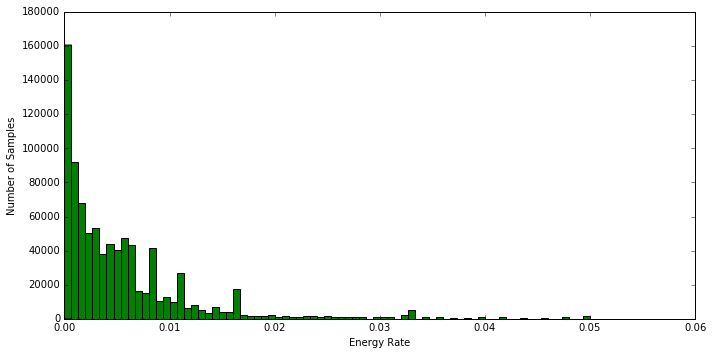
\includegraphics[width=\textwidth]{images/carat-data/energy_rate.png}
%	\caption{Histogram of energy rates with 75 bins}
%	\label{figure:carat-data-energy-rate}
%\end{figure}  
\begin{figure} %[!htbp]
	\centering
	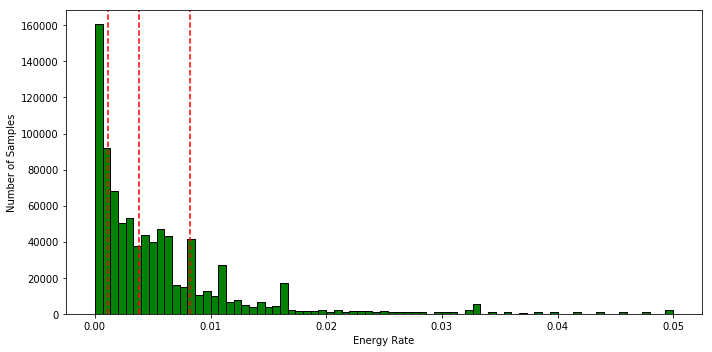
\includegraphics[width=\textwidth]{images/carat-data/energy_rate_w_boundaries.png}
	\caption{Histogram of energy rates with 75 bins in green. The dotted red lines show the boundaries of the four equal mass bins.}
	\label{figure:carat-data-energy-rate}
\end{figure}  


Figure~\ref{figure:carat-data-energy-rate} shows a histogram of the energy rate distribution. The distribution appears to be a rough approximation of an exponential distribution. The distribution does not seem have an evident categorical division. Thus, the data was discretized by dividing it to four bins of equal mass. The discretization boundary points along the energy rate -axis were 0.0011, 0.0038 and 0.0083.

\subsection{CPU Usage Level} \label{carat data cpu} 

CPU usage level is the fraction of time that the central processing unit(s) of the mobile device were busy when the sample was collected. The CPU usage level is in a unit of percentages of the maximum level. All CPU usage levels that were below zero or greater than 1 were discarded as faulty data.

%\begin{figure} %[!htbp]
%	\centering
%	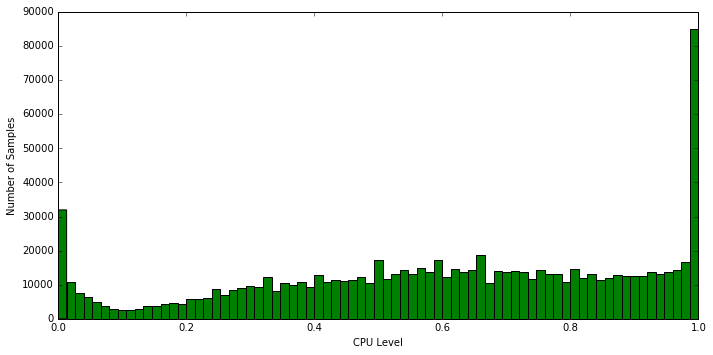
\includegraphics[width=\textwidth]{images/carat-data/cpu_level.png}
%	\caption{Histogram of CPU usage levels with 75 bins}
%	\label{figure:carat-data-cpu-level}
%\end{figure}  
\begin{figure} %[!htbp]
	\centering
	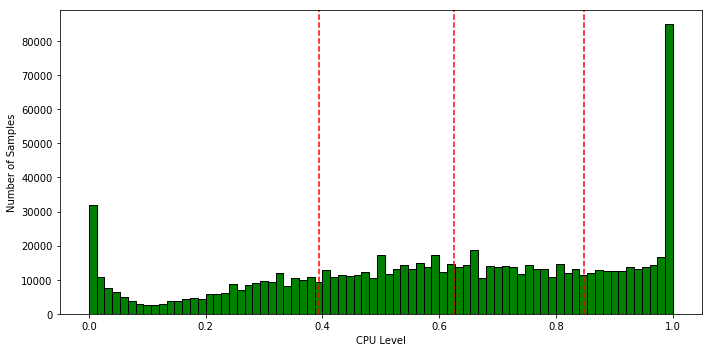
\includegraphics[width=\textwidth]{images/carat-data/cpu_level_w_boundaries.png}
	\caption{Histogram of CPU usage levels with 75 bins in green. The dotted red lines show the boundaries of the four equal mass bins.}
	\label{figure:carat-data-cpu-level}
\end{figure} 

Figure~\ref{figure:carat-data-cpu-level} shows a histogram of the CPU usage level distribution. The distribution very roughly approximates the uniform distribution except for 100\% and 0\% CPU usage levels, which are quite overrepresented. The data was discretized into four bins of equal frequency. The discretization boundary points along the CPU usage -axis were 0.39, 0.63 and 0.85. 

High CPU usage rate has been shown to increase the level mobile device energy consumption~\cite{5375354, PELTONEN201671}, and has been identified as one of the most significant variables in predicting a device's energy consumption. One would therefore assume the CPU utilization level to appear as an antecedent for rules which predict high energy consumption.    

\subsection{Travel Distance}  

Travel distance is the distance in meters, that the mobile device moved between the two samples. Moving mobile phone users have been shown to consume less energy on average compared to stationary ones~\cite{7146507}. This could be due to stationary users being more likely to actively use their devices. 

\begin{figure} %[!htbp]
	\centering
	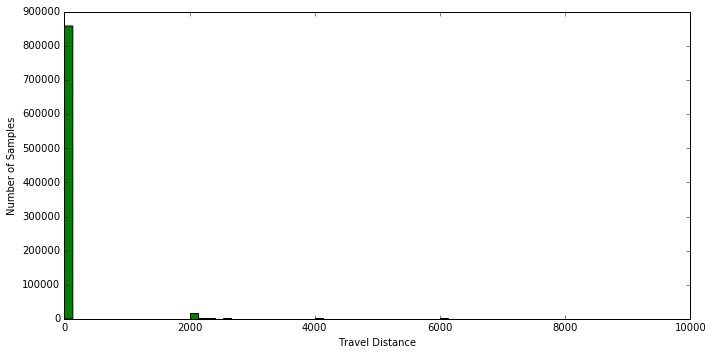
\includegraphics[width=\textwidth]{images/carat-data/travel_distance.png}
	\caption{Histogram of travel distance with 75 bins}
	\label{figure:carat-data-travel-distance}
\end{figure}  

Figure~\ref{figure:carat-data-travel-distance} shows a histogram of the travel distance distribution. Most of the mass of the distribution is concentrated in the close proximity of zero with other values having very low frequencies. The travel distance was discretized to two categories: \textit{moving}, if the travelled distance was greater than 100 meters, and \textit{static} otherwise.

\subsection{Battery Temperature}  

Battery temperature is the measured mobile device battery temperature in degrees Celsius. Temperatures less than five degrees were discarded as it is very rare for a battery temperature to be that low even in subzero climates. Likewise battery temperatures of over 100 degrees were discarded, as healthy devices very rarely reach such high battery temperatures.

%\begin{figure} %[!htbp]
%	\centering
%	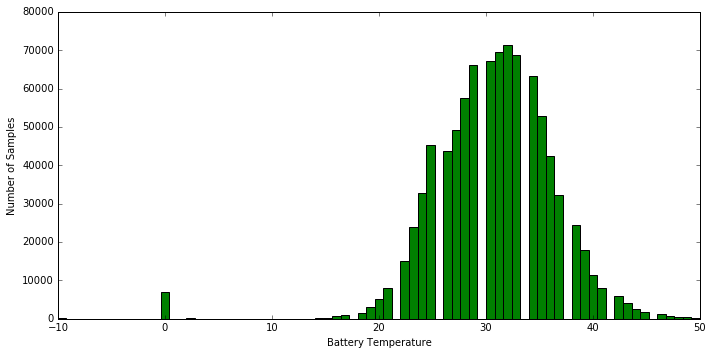
\includegraphics[width=\textwidth]{images/carat-data/battery_temperature.png}
%	\caption{Histogram of battery temperatures with 75 bins}
%	\label{figure:carat-data-battery-temperature}
%\end{figure}  
\begin{figure} %[!htbp]
	\centering
	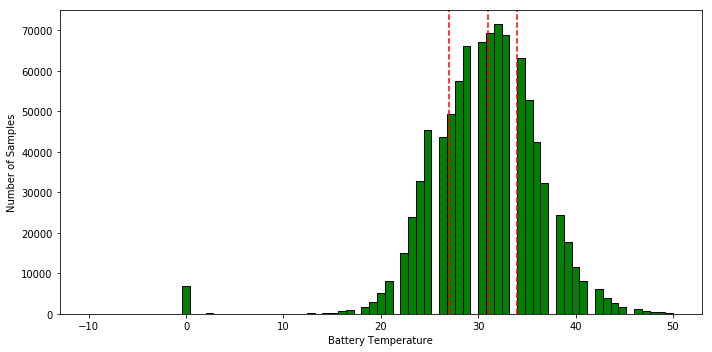
\includegraphics[width=\textwidth]{images/carat-data/battery_temperature_w_boundaries.png}
	\caption{Histogram of battery temperatures with 75 bins in green. The dotted red lines show the boundaries of the four equal mass bins.}
	\label{figure:carat-data-battery-temperature}
\end{figure}

Figure~\ref{figure:carat-data-battery-temperature} shows a histogram of the battery temperature distribution. The distribution approximates a normal distribution with some skewedness. Notably, there is a small cluster of measurements near zero degrees Celsius. This is most likely due to mobile devices systematically reporting a value of zero if the measurement data is not available. The data was discretized into four bins of equal frequency. The discretization boundary points along the battery temperature -axis were 27, 31 and 34. 

High battery temperature has been shown to cause increased battery consumption~\cite{7146507}. The increase in battery temperature cannot always be explained by CPU usage alone, and other factors such as the ambient temperature can affect the battery temperature. It is to be expected that high battery temperature appears as an antecedent of many rules predicting very high energy consumption.
%A straightforward hypothesis would be that a higher battery temperature leads to increased energy rate.

\subsection{Battery Voltage}  

Battery voltage is the electric potential difference generated by the battery in units of volts. Different devices may carry batteries with different voltages. A malfunctioning battery that is near end of its lifetime may give lower than usual voltage readings.

%\begin{figure} %[!htbp]
%	\centering
%	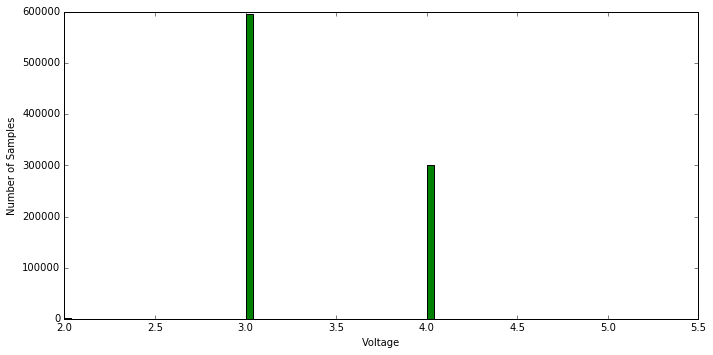
\includegraphics[width=\textwidth]{images/carat-data/battery_voltage.png}
%	\caption{Histogram of battery voltages with 75 bins in green.}
%	\label{figure:carat-data-battery-voltage}
%\end{figure}  
\begin{figure} %[!htbp]
	\centering
	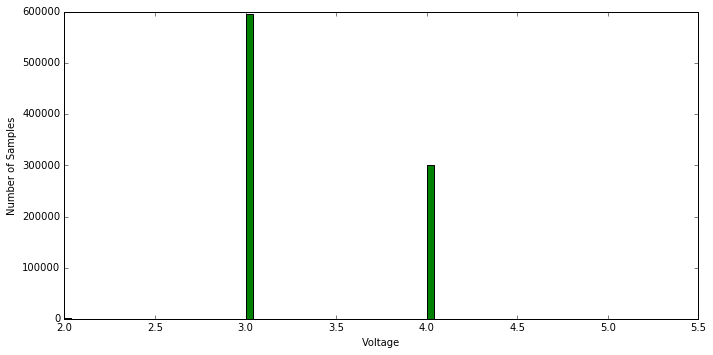
\includegraphics[width=\textwidth]{images/carat-data/battery_voltage.png}
	\caption{Histogram of battery voltages with 75 bins in green.}
	\label{figure:carat-data-battery-voltage}
\end{figure}

Figure~\ref{figure:carat-data-battery-voltage} shows a histogram of battery voltage distribution from the Carat data. The voltages are clustered almost discretely around values of 2, 3 and 4 volts. The voltages were accordingly divided to three bins to reflect this clustering. The discrete voltage data is due to a bug in the Carat data collection software which rounds the readings to integer values. This bug affects the data set used in this thesis work, but has since been fixed. By using a more recent dataset, one would be able to use continuous battery voltage readings in the analysis, which would likely increase the predictive power and accuracy of the generated association rules.         

\subsection{Screen Brightness} \label{carat data screen}

Screen brightness is system setting that takes integer values between -1 and 255. Higher values correspond to higher screen brightness. The value negative one has a special meaning indicating automatic screen brightness, where the screen's brightness is adjusted according to changing illumination of the environment~\cite{PELTONEN201671}.

%\begin{figure} %[!htbp]
%	\centering
%	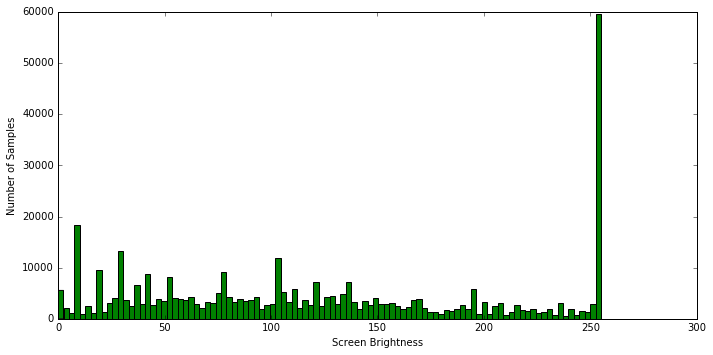
\includegraphics[width=\textwidth]{images/carat-data/screen_brightness.png}
%	\caption{Histogram of screen brightness divided to 100 bins}
%	\label{figure:carat-data-screen-brightness}
%\end{figure}
\begin{figure} %[!htbp]
	\centering
	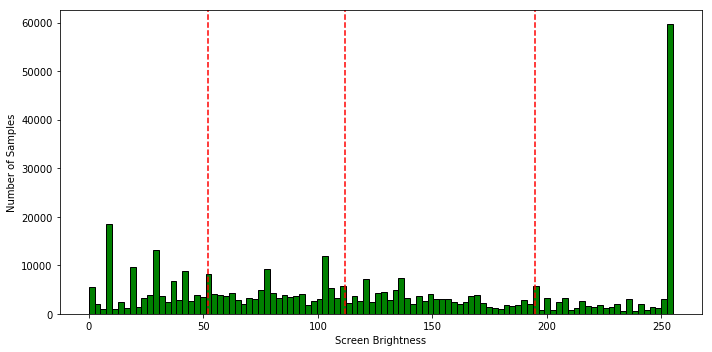
\includegraphics[width=\textwidth]{images/carat-data/screen_brightness_w_boundaries.png}
	\caption{Histogram of screen brightness divided to 100 bins in green. The dotted red lines show to boundary points of the four equal mass bins.}
	\label{figure:carat-data-screen-brightness}
\end{figure}     

Figure~\ref{figure:carat-data-screen-brightness} shows a histogram of the screen brightness values, where the values of -1 have been removed. The brightness values seem to roughly follow a uniform distribution, although very high screen brightness settings seem to be over represented. Approximately half of the samples had their brightness value at -1, indicating automatic brightness setting. Since the automatic setting is categorically different from all other brightness values, the brightness attribute was discretized in the following way: the value -1 formed it's own bin labelled as "auto", while the other numerical values were divided to four bins of equal mass. The boundary points of the equal mass bins along the screen brightness -axis were 52, 112 and 195.   

Increase in screen brightness has been shown to cause increased energy consumption in mobile devices~\cite{5375354, PELTONEN201671} while low and automatically adjusted screen brightness values lead to decrease in energy consumption. It is expected that this phenomena shows up in the association rules as well.

\subsection{Mobile Network Technology}  

The mobile network technology is a system property that reports the name of the mobile technology that mobile device is using for its mobile data communication. Common values include LTE, HSPA, EDGE and UTMS.

\begin{figure} %[!htbp]
	\centering
	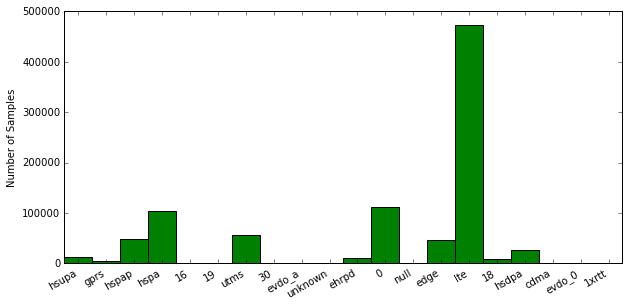
\includegraphics[width=\textwidth]{images/carat-data/mobile_net_type.png}
	\caption{Histogram of mobile network technologies in Carat data.}
	\label{figure:carat-data-mobile-net-type}
\end{figure}   

Figure~\ref{figure:carat-data-mobile-net-type} shows a histogram of all mobile network types in the Carat data. Numeric values were mapped to mobile network type names according to Android developer reference manual~\footnote{https://developer.android.com/reference/android/telephony/TelephonyManager.html}. Ambiguous values such as "unknown", "null" as well as any numerical value not listed in the Android developer reference manual, were combined to a single bin labelled as "unknown". 

Different mobile networking technologies have been shown to have varying energy consumption performance depending on the task~\cite{5357972}. Based on this observation, one would assume that different mobile network technologies should appear as antecedents for association rules predicting either high or low energy consumption depending on the network usage pattern of the mobile application.  

%Intuitively, one would assume that older mobile network technologies such as \textit{gprs} would consume less battery life than newer technologies such as \textit{lte}, since the newer technologies achieve much greater data rates than the old technologies.

\subsection{Network Type}  

Network type is a system property that is reported by the mobile device to indicate the type of the data connection. Typically this is either \textit{mobile} or \textit{wifi}, indicating the use of mobile networking or a wireless local area networking respectively. Some more exotic alternatives can however be found in the data, such as \textit{bluetooth tethering}, where the network access is enabled by bluetooth tunneling through another device.

\begin{figure} %[!htbp]
	\centering
	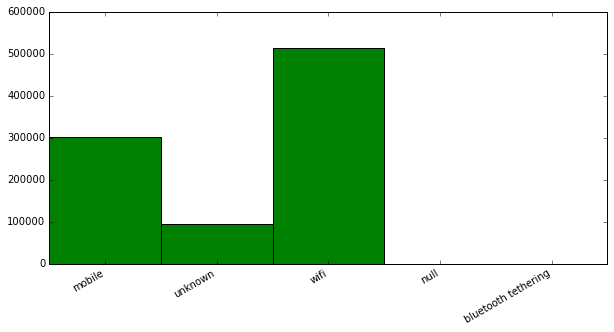
\includegraphics[width=\textwidth]{images/carat-data/network_type.png}
	\caption{Histogram of network types in Carat data}
	\label{figure:carat-data-net-type}
\end{figure}   

Figure~\ref{figure:carat-data-net-type} shows a histogram of all network types found in the Carat data. Values \textit{null} and \textit{unknown} were considered ambiguous and were combined under the label \textit{unknown}.
 
The choice of networking technology has been shown to affect the energy consumption of mobile devices~\cite{7146507, 6240745}. As a general rule, using WiFi network for downloading data is more energy efficient than using a mobile networking technology. Therefore a reasonable hypothesis is to expect to see association rules with mobile networking type as an antecedent for rules predicting high energy consumption, at least in case of applications that download a lot of data.  

\subsection{WiFi Signal Strength}

WiFi signal strength is a system property that the mobile device uses to signify the strength of the wireless local area network. WiFi connection strength is reported as an integer value in the range -100 to 0, where 0 signifies the strongest signal. Presumably, the WiFi signal strength is in units of decibels relative to milliwatt (dBm). The Android API seems to report a value of -127 when no reading is available. Values less than -100 were excluded from the data as these are very unlikely to be real measurements.

% \begin{figure} %[!htbp]
%	\centering
%	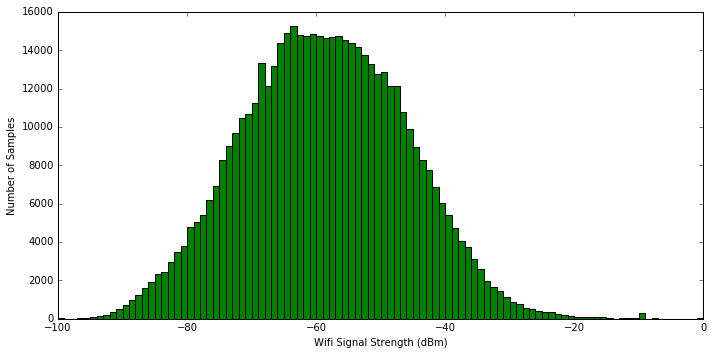
\includegraphics[width=\textwidth]{images/carat-data/wifi_signal_strength.png}
%	\caption{Histogram of WiFi signal strengths readings with 100 bins in Carat data}
%	\label{figure:carat-data-wifi-signal-strength}
%\end{figure}
\begin{figure} %[!htbp]
	\centering
	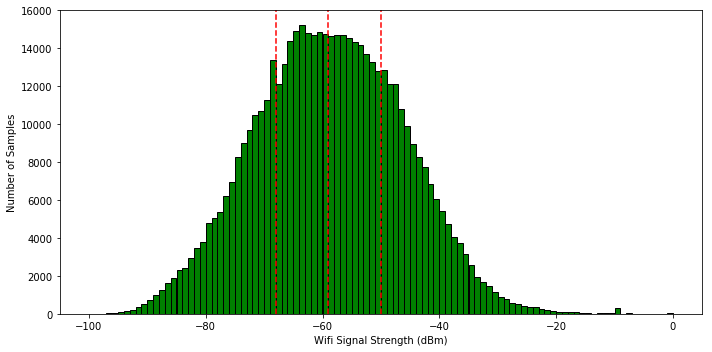
\includegraphics[width=\textwidth]{images/carat-data/wifi_signal_strength_w_boundaries.png}
	\caption{Histogram of WiFi signal strengths readings with 100 bins in green. The dotted red lines show the boundaries of the four equal mass bins.}
	\label{figure:carat-data-wifi-signal-strength}
\end{figure} 

Figure~\ref{figure:carat-data-wifi-signal-strength} shows a histogram of WiFi signal strengths in Carat data. The distribution seems to approximate a normal distribution reasonably well. The data was discretized in four bins with equal mass, the boundaries of which were -68.0, -59.0 and -50.0.

Poor WiFi signal strength has been shown to decrease battery life of mobile devices~\cite{7146507}. This is likely due to increase in the noisiness of the connection, leading to increased data loss and retransmissions, which require extra energy. This effect is expected to be seen in the association rules generated for applications that rely heavily on networking.
%One hypothesis for the interactions between the signal strength and energy rate would be that lower signal strength leads to higher energy rate, as low signal strength s generally increase the noisiness of the connection, leading to increased data loss and retransmissions, which require extra battery life.

\subsection{WiFi Link Speed}

WiFi link speed is a system property that the mobile device uses to report the current wireless local area network link speed. The link speed is presumably reported in units of mega bits per second (mbps). 

WiFi link speed has been shown to have an impact on the mobile device energy consumption~\cite{7146507, 5375354}. Increase in link speed seems to lead to an increase in energy consumption, although this connection does not appear to be nearly as significant as WiFi signal strength for example. The slight increase in energy consumption might be due to users with faster link being able to consume downloadable content more quickly, thus draining the battery more efficiently.
%\begin{figure} %[!htbp]
%	\centering
%	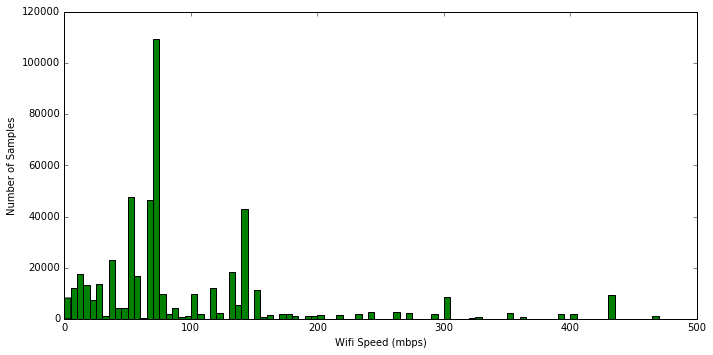
\includegraphics[width=\textwidth]{images/carat-data/wifi_speed.png}
%	\caption{Histogram of WiFi link speed with 100 bins in Carat data}
%	\label{figure:carat-data-wifi-speed}
%\end{figure}

Figure~\ref{figure:carat-data-wifi-speed} shows a histogram of the WiFi link speeds in the Carat data. The link speeds were divided to four bins of equal mass. The boundary points of the bins along the link speed -axis were 54.0, 72.0 and 130.0. 

\begin{figure} %[!htbp]
	\centering
	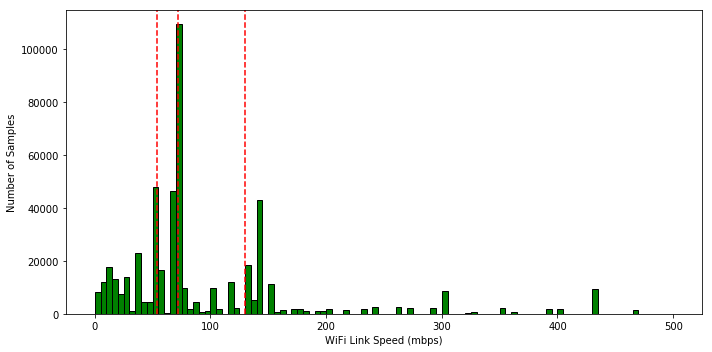
\includegraphics[width=\textwidth]{images/carat-data/wifi_speed_w_boundaries.png}
	\caption{Histogram of WiFi link speed with 100 bins in green. The dotted red lines show the boundary points of the four equal mass bins.}
	\label{figure:carat-data-wifi-speed}
\end{figure}